\chapter[Capítulo 4. Diseño del Hardware ]{Diseño del Hardware.}

\section{PIC (Peripheral Interface Controller)}

Los PIC son una familia de microcontroladores  fabricados por Microchip Tecnhnology Inc. Para el control y proceso del manejo del protocolo BUS CAN en nuestra placa electrónica se escoge este tipo de microcontrolador debido a su sencillo manejo y programación, además de su bajo costo y la documentación de usuarios que hay detrás de este microcontrolador. Los PIC no son los microcontroladores con más prestaciones pero sus características se ajustan al proyecto. Existe una gran cantidad de modelos de PIC con características y prestaciones. Esto nos permite escoger el modelo que se ajusta a la necesidad. 

Para que el PIC pueda realizar sus funciones es necesario programarlo y hemos de escribir un programa que contenga los procesos que el PIC debe ejecutar para leer el protocolo BUS CAN. Este programa se puede escribir en varios lenguajes de programación, pero los  más utilizados son el ’Assembler’ (ensamblador) y el C. En el proyecto se utiliza el lenguaje C por su potencia y robustez para sistemas embebidos, para un último paso y traducir el programa a lenguaje máquina se utiliza el compilador  de CCS (Custom Computer Services, Inc.)

Como todo microcontrolador, el PIC se puede dividir en diferentes bloques:
\begin {itemize}

\item {\textbf{Reloj:}}  Para sincronizar las instrucciones del sistema todos los PIC necesitan un circuito oscilador que genere una onda cuadrada de alta frecuencia, para ello tiene incorporado un oscilador interno de baja frecuencia y para mayor margen de frecuencia se utiliza un circuito externo con cristal de cuarzo, resonador cerámico o una red RC (resistencia y capacitor). 
\item {\textbf{(In/Out):}} Los  pines que posee un PIC son configurables como entrada o salida de señales binarias.
\item {\textbf{CPU:}} la CPU (Central Processing Unit, por sus siglas en inglés) es el encargado de interpretar las instrucciones y quien procesa los datos en los programas del PIC. 
\item {\textbf{Memoria de datos:}} contiene memoria RAM (Random Access Memory, por sus siglas en inglés) de lectura y escritura además de contar con memoria del tipo EEPROM (Electrically-Erasable Programmable Read-Only Memory, por sus siglas en inglés). Con la memoria EEPROOM un corte en el suministro de la alimentacion no ocasiona la pérdida de datos almacenados al reiniciarse el programa del PIC. 
\item {\textbf{}{Memoria de programas:}} Existen varios tipos de memoria adecuados para soportar estas funciones, de las cuales en los PIC se utilizan la ROM (Read-Only Memory, por sus siglas en inglés), OTP (One-Time Programmable, por sus siglas en inglés) y Flash. 
\item {\textbf{Periféricos:}} Se llama periféricos a todas aquellas unidades con la cual el PIC se comunica con el mundo exterior como por ejemplo el  ADC (Analog to Digital Converter, por sus siglas en inglés),  los comparadores, temporizadores, EUSART (Enhanced Universal Synchronous Asynchronous Receiver Transmitter, por sus siglas en inglés), USB (Universal Serial Bus, por sus siglas en inglés), MSSP (Master Synchronous Serial Port, por sus siglas en inglés) que permite manejar los protocolos I2C y SPI, CAN (Controller Area Network, por sus siglas en inglés) y los módulos CCP/ECCP (Enhanced Capture/Compare/PWM, por sus siglas en inglés) los cuales se pueden utilizar como comparador, como capturador o como PWM (Pulse-Width Modulation, por sus siglas en inglés).
\end{itemize}

Conocidas algunas características de los PICs conoceremos las especificaciones del PIC a utilizar en nuestro sistema. El microcontrolador es el PIC18F4580 el cual soporta los módulos CAN y EUSART cuyas características son las siguientes:
\begin{itemize}
\item {\textbf{Reloj:}} Ofrece varias opciones de configuración de la frecuencia de oscilación, permitiendo al usuario escoger según se adapte a sus necesidades:
Para la elección de la frecuencia de oscilación, el fabricante nos ofrece unas tablas:
Los condensadores elegidos van del pin OSC1 o OSC2 a 0V (GND). En el diseño de nuestra placa hemos escogido como frecuencia de oscilación 20 MHz.
\item {\textbf{Input/Output:}} En este PIC hay 5 puertos diferentes (A, B, C, D y E). Cada puerto tiene tres registros para sus operaciones que son el TRIS (registro de dirección de datos), el PORT (el que lee el nivel de tensión que hay en el pin) y el LAT (utilizado en operaciones lectura-modificación-escritura del valor que el pin I/O está leyendo). 

\item {\textbf{Memoria de datos:}} Tiene 1536 bytes de memoria RAM y 256 bytes de EEPROM.
\item {\textbf{Memoria de programa:}} Tiene 32 kbytes de memoria Flash.
\item {\textbf{Periféricos:}} En el PIC18F4580 podemos encontrar 11 ADC de 10 bits, dos módulos CCP/ECCP, MSSP para I2C y SPI, EUSART, dos comparadores, 4 temporizadores (uno de 8 bits y tres de 16 bits) y un modulo CAN,\cite{DaP}.

\end{itemize}

\subsection{Módulo CAN del PIC 18F4580}
Las características del módulo son los siguientes:
\begin{itemize}
\item Aplicación del protocolo CAN 1.2,
CAN 2.0A y CAN 2.0B.
\item Tramas de datos estándar y extendidas.
\item 0-8 bytes de longitud de datos.
\item Tasa de bits programable hasta 1 Mbit / seg.
\item Totalmente compatible con módulos CAN PIC18XXX8.
\item Tres modos de funcionamiento:
	\begin{itemize}
    	\item Modo 0: El modo tradicional.
		\item Modo 1: Mejora del modo tradicional con
apoyo DeviceNet.
		\item Modo 2: Modo FIFO con el apoyo de DeviceNet.
	\end {itemize}
\item Soporte para tramas remotas con el manejo automatizado.
\item  Seis memorias intermedias programables como RX y TX, 
almacenamientos intermedios de mensajes.
\item 16 filtros de aceptancia.
\item Dos máscaras de filtro de aceptancia completos que pueden ser asignado a cualquier filtro.
\item Tres buffers de transmisión dedicados.
\item Temporizador interno,\cite{DaP}.
\item Modo de bajo consumo.
\end{itemize}

\subsection{Transceiver BUS CAN }
Están diseñados para uso en aplicaciones de comunicación BUS CAN en la capa física según la norma ISO 11898. El transceiver proporciona una transmisión y recepción de bus diferencial para el controlador CAN y ofrece velocidades de hasta 1Mbps.
Diseñado para funcionar en ambientes agresivos este dispositivo cuenta con protección contra sobretensiones, sobrecalentamiento y una amplia gama de modos de servicios. El pin 8 ofrece tres modos de funcionamiento: alta velocidad, control de pendiente, y modos de bajo consumo.
El modo de alta velocidad de funcionamiento se selecciona mediante la conexión del PIN 8 a tierra, permitiendo a los transistores de salida del transmisor encender y apagar lo más rápido posible.
Las pendientes de subida y bajada de los bits se pueden ajustar mediante la conexión de una resistencia a tierra en el PIN 8, ya que la pendiente del bit es proporcional a la corriente de salida del PIN. Este control de la pendiente se implementa aplicando valores a la resistencia externa en el PIN 8. Por ejemplo con una resistencia de 10 kohm se logra una pendiente de bit de 15V/us,  y con una resistencia de 100 kohm se logra una pendiente de bit de 2V/us. Si se aplica un nivel lógico alto al PIN 8 el transceiver entra en modo standby, para ahorrar energía y vuelve a su estado de trabajo al aplicar un nivel lógico bajo al PIN 8.

El pin Vref 5 está disponible como una referencia de tensión, \cite{sn}.

\subsection{Diseño del Hardware}
El montaje implementado es una placa de hardware BUS CAN, basado en el microcontrolador de bajo coste PIC18F4580. La función principal del mismo, es poder leer datos del BUS
CAN y enviarlos a un servidor para mostrarlos en una interfaz gráfica. Para realizar la placa PCB (Printed Circuit Board, por sus siglas en inglés) se utilizó el software EAGLE (Easily Applicable Graphical Layout Editor, por sus siglas en inglés) el cual es un programa de diseño de diagramas y PCBs con autoenrutador. Muchas versiones de este programa tienen una licencia Freeware y gran cantidad de bibliotecas de componentes alrededor de la red de internet. Eagle tiene una facilidad de uso y configuración.

En la \textbf{Figura \ref{Esch1}} se observa el diagrama del bloque de alimentación del hardware que cuenta con un regulador de tensión LM7805 y dos condensadores electrolíticos cuya función es eliminar el rizado de la señal en la entrada del regulador para que la tensión de salida no tenga variaciones de tensión debido a irregularidades de la fuente principal. 

%%%%%%%%%%%%%%%%%%%%%%%%%%%%%%%%%%%%%%%%%%%%%%%%%%%%%%%%%%
\begin{figure}[H]
	\centering
		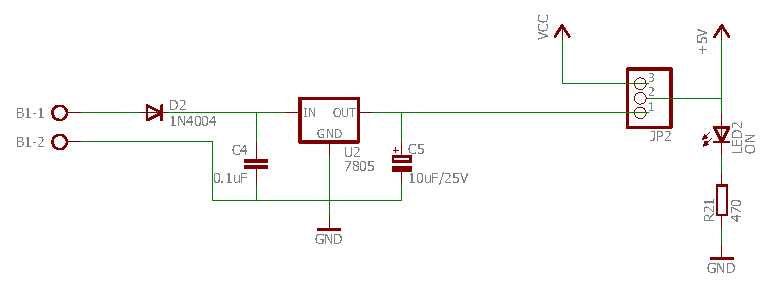
\includegraphics[width=0.8\textwidth]{./Cap4imagen/Fuente.pdf}
	\caption[Fuente de Alimentación.]{Fuente de Alimentación.\textbf{ Fuente:} \cite{sch1}.}
	\label{Esch1} % Etiqueta para la referencia.
\end{figure}

% CITAR IMAGEN


%%%%%%%%%%%%%%%%%%%%%%%%%%%%%%%%%%%%%%%%%%%%%%%%%%%%%%%%%%
El Diagrama principal contiene el microncontrolador PIC18F4580 el cual se muestra en la \textbf{Figura \ref{Esch2}} el cual será el nodo maestro encargado de escanear  y procesar los datos provenientes del bus.En la \textbf{Figura \ref{Esch3}} se observa los conectores de la placa de manera a hacerla escalable y tener opciones de conexión para las salidas de las señales. El mismo fue desarrollado en una capa y las pistas que no se pudieron enrutar se comunican con puentes. En la \textbf{Figura \ref{Esch5}} se puede ver la imagen en PCB y en la \textbf{Figura \ref{Esch6}} se observa la distribución de los componentes electrónicos en la placa.


%%%%%%%%%%%%%%%%%%%%%%%%%%%%%%%%%%%%%%%%%%%%%%%%%%%%%%%%%%%
\begin{figure}[H]
	\centering
		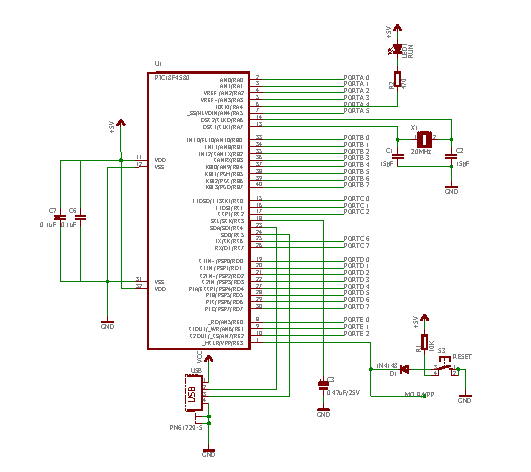
\includegraphics[width=0.8\textwidth]{./Cap4imagen/PIC.pdf}
	\caption[Esquemático del PIC.]{Esquemático del PIC.\textbf{ Fuente:} \cite{Tu}.}
	\label{Esch2} % Etiqueta para la referencia.
\end{figure}

% CITAR IMAGEN


%%%%%%%%%%%%%%%%%%%%%%%%%%%%%%%%%%%%%%%%%%%%%%%%%%%%%%%%%%%

%%%%%%%%%%%%%%%%%%%%%%%%%%%%%%%%%%%%%%%%%%%%%%%%%%%%%%%%%%%%%
\begin{figure}[H]
	\centering
		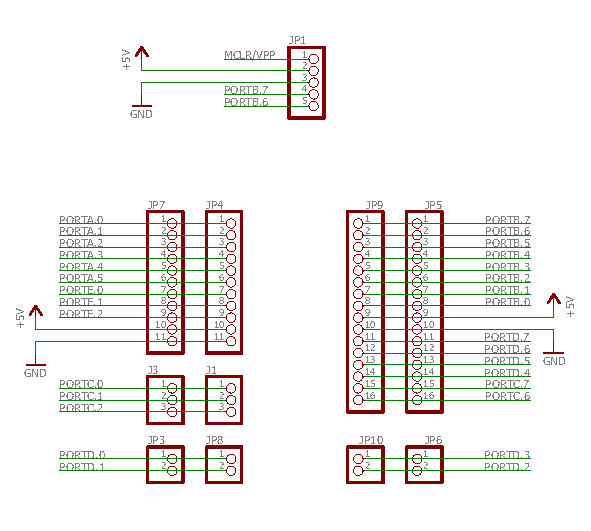
\includegraphics[width=0.8\textwidth]{./Cap4imagen/Conectores.pdf}
	\caption[Conectores del Hardware.]{Conectores del Hardware.\textbf{ Fuente:} \cite{Tu}.}
	\label{Esch3} % Etiqueta para la referencia.
\end{figure}

% CITAR IMAGEN


%%%%%%%%%%%%%%%%%%%%%%%%%%%%%%%%%%%%%%%%%%%%%%%%%%%%%%%%%%%%%
%%%%%%%%%%%%%%%%%%%%%%%%%%%%%%%%%%%%%%%%%%%%%%%%%%%%%%%%%%%%%

%%%Las distancias indicadas son trim = izquierda abajo
%%%derecha arriba, y debe ir siempre seguido del comando clip.
\begin{figure}[H]
	\centering
		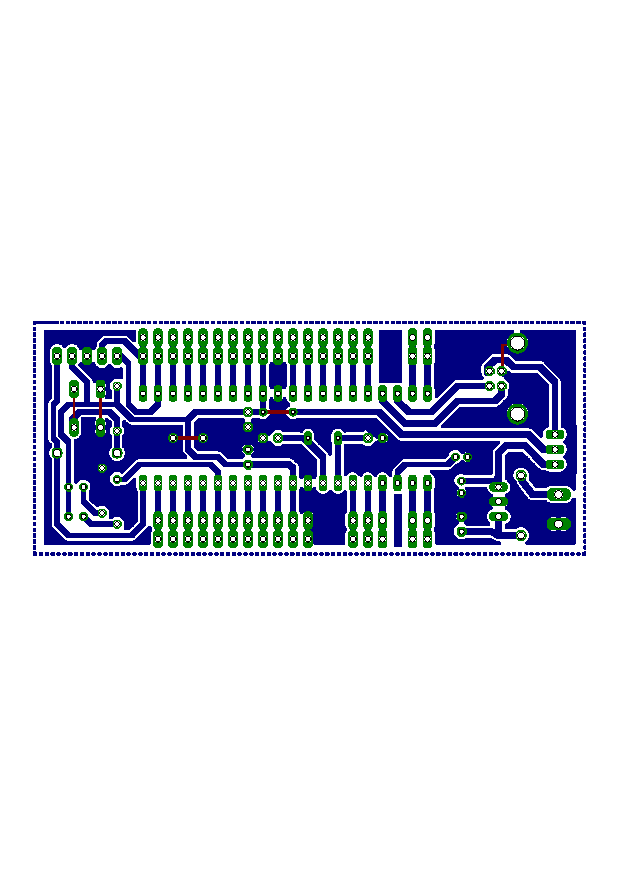
\includegraphics[trim = 5mm 53mm 5mm 50mm, clip, width=0.8\textwidth]{./Cap4imagen/CanPcb8.pdf}
	\caption[Diseño PCB de la Placa BUS CAN.]{Diseño PCB de la Placa BUS CAN.\textbf{ Fuente:} \cite{Tu}.}
	\label{Esch5} % Etiqueta para la referencia.
\end{figure}

% CITAR IMAGEN


%%%%%%%%%%%%%%%%%%%%%%%%%%%%%%%%%%%%%%%%%%%%%%%%%%%%%%%%%%%%%
\begin{figure}[H]
	\centering
		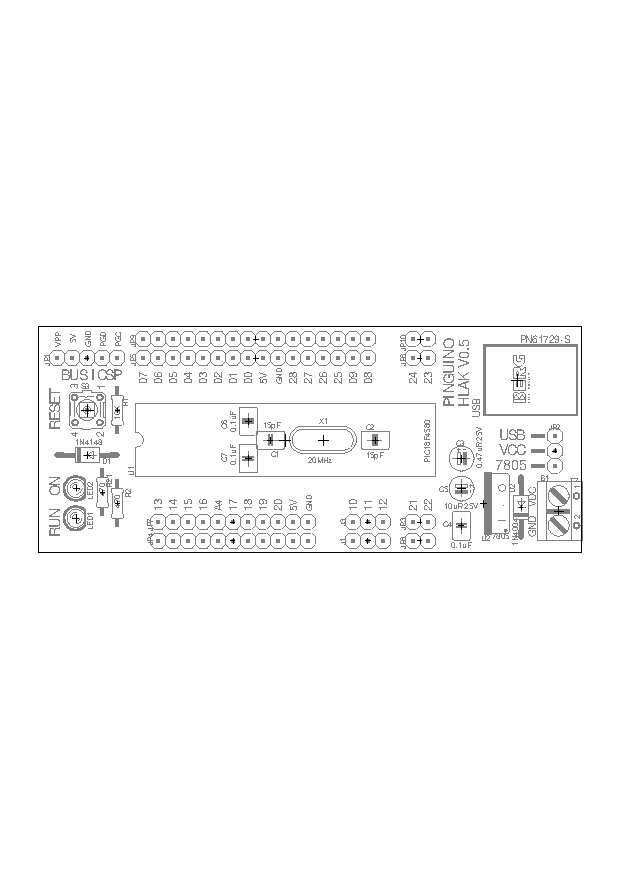
\includegraphics[trim = 5mm 53mm 5mm 50mm, clip, width=0.8\textwidth]{./Cap4imagen/CanGraf2.pdf}
	\caption[ Ubicación de Componentes en el PCB BUS CAN.]{Ubicación de Componentes en el PCB BUS CAN.\textbf{ Fuente:} \cite{Tu}.}
	\label{Esch6} % Etiqueta para la referencia.
\end{figure}

% CITAR IMAGEN


%%%%%%%%%%%%%%%%%%%%%%%%%%%%%%%%%%%%%%%%%%%%%%%%%%%%%%%%%

El Transceiver 65HVD251 de Texas Instruments es una interfaz entre el controlador del protocolo BUS CAN que se encuentra en el PIC, y el BUS CAN físico. Este chip está formado por un driver que nos convierte las señales que entran por el CANH  y CANL a señales CMOS para tener una lectura correcta de los datos en el PIC. La configuración de pines se muestra en la \textbf{Figura \ref{Esch4}}, su montaje contiene tres resistencias en serie para dar un valor de 17kohm y no requiere otros elementos aparte de los propios conectores para  entrada, salida y fuente de alimentación.
En la \textbf{Figura \ref{Esch7}} se muestra el circuito PCB del mismo y en la \textbf{Figura \ref{Esch8}} la disposición de los componentes electrónicos de la placa.

%%%%%%%%%%%%%    TRANSEIVER         %%%%%%%%%%%%%%%%%%%
\begin{figure}[H]
	\centering
		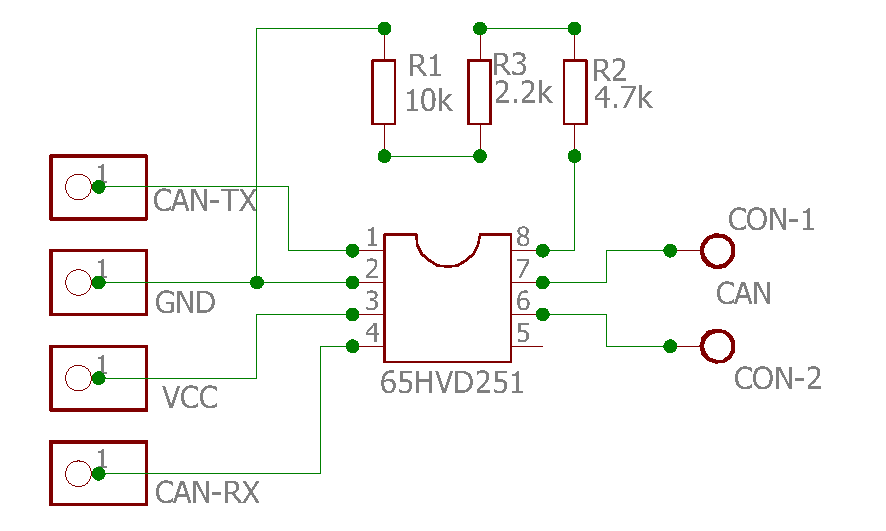
\includegraphics[width=0.8\textwidth]{./Cap4imagen/transSchem.pdf}
	\caption[Esquemático del Transceiver BUS CAN.]{Esquemático del Transceiver BUS CAN.\textbf{ Fuente:} \cite{DaP}.}
	\label{Esch4} % Etiqueta para la referencia.
\end{figure}

% CITAR IMAGEN


%%%%%%%%%%%%%%%%%%%%%%%%%%%%%%%%%%%%%%%%%%%%%%%%%%%%%%%%%%%%%

%%%%%%%%%%%%%%%%%%%%%%%%%%%%%%%%%%%%%%%%%%%%%%%%%%%%%%%%%%%%%
\begin{figure}[H]
	\centering
		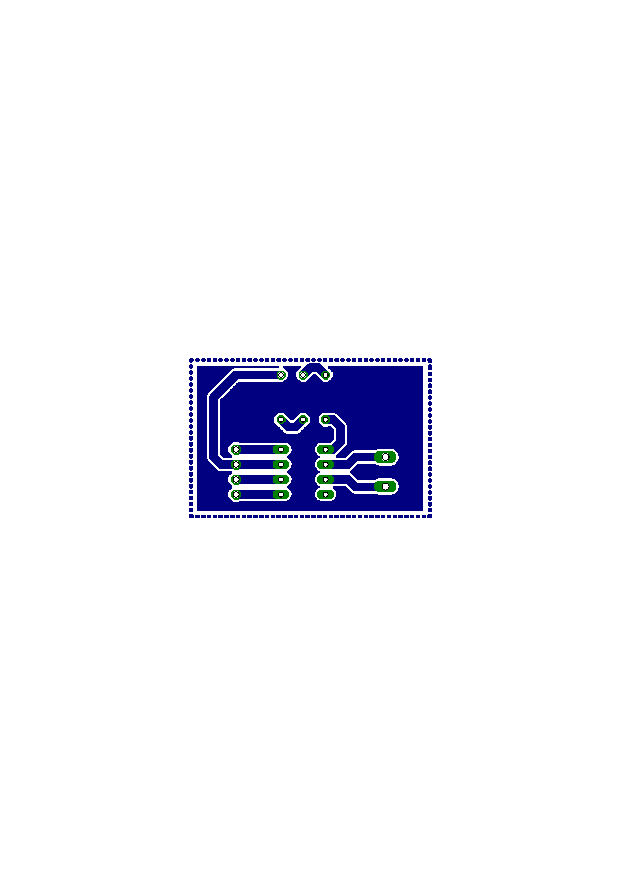
\includegraphics[trim = 5mm 60mm 5mm 60mm, clip, width=0.8\textwidth]{./Cap4imagen/transPcb3.pdf}
	\caption[PCB del Transceiver BUS CAN.]{PCB del Transceiver BUS CAN.\textbf{ Fuente:} \cite{DaP}.}
	\label{Esch7} % Etiqueta para la referencia.
\end{figure}

% CITAR IMAGEN


%%%%%%%%%%%%%%%%%%%%%%%%%%%%%%%%%%%%%%%%%%%%%%%%%%%%%%%%%

%%%%%%%%%%%%%%%%%%%%%%%%%%%%%%%%%%%%%%%%%%%%%%%%%%%%%%%%

\begin{figure}[H]
	\centering
		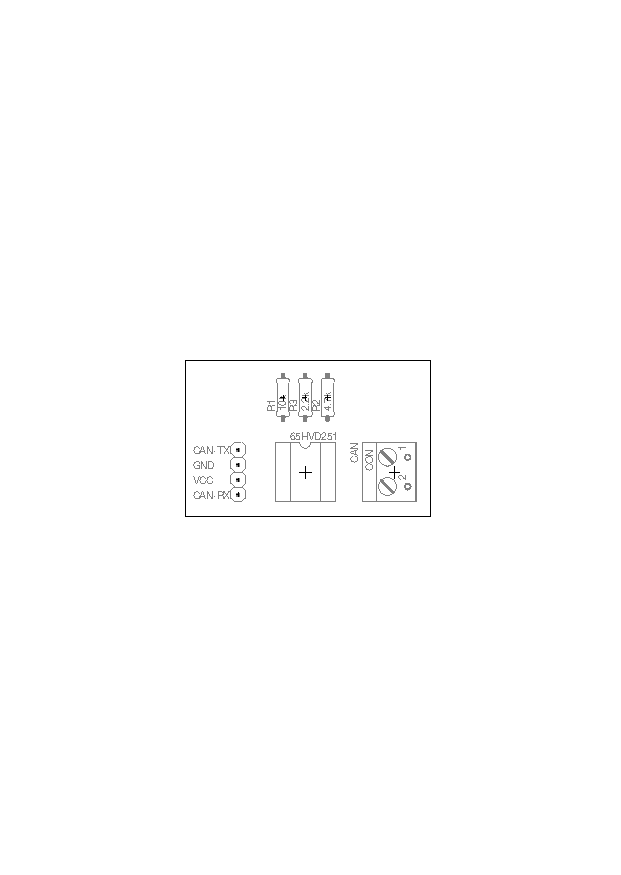
\includegraphics[trim = 5mm 60mm 5mm 60mm, clip, width=0.8\textwidth]{./Cap4imagen/transGraf1.pdf}
	\caption[Ubicación de Componentes en el PCB del Transceiver BUS CAN.]{Ubicación de Componentes en el PCB del Transceiver BUS CAN.\textbf{ Fuente:} \cite{DaP}.}
	\label{Esch8} % Etiqueta para la referencia.
\end{figure}

% CITAR IMAGEN


%%%%%%%%%%%%%%%%%%%%%%%%%%%%%%%%%%%%%%%%%%%%%%%%%%%%%%